\title{CS 5780: HW3}
\author{
        Kimberly Sheriff, kgs45\\
      	Brian Toth, bdt25
}
\date{\today}

\documentclass[12pt]{article}

\usepackage{graphicx}
\usepackage[margin=1in]{geometry}
\usepackage{color}
\usepackage{amssymb}
 \usepackage{latexsym}
\usepackage{subfigure}



\usepackage{listings}
\lstset{ %
language=C,                % choose the language of the code
basicstyle=\footnotesize,       % the size of the fonts that are used for the code
numbers=left,                   % where to put the line-numbers
numberstyle=\footnotesize,      % the size of the fonts that are used for the line-numbers
stepnumber=1,                   % the step between two line-numbers. If it is 1 each line will be numbered
numbersep=5pt,                  % how far the line-numbers are from the code
backgroundcolor=\color{white},  % choose the background color. You must add \usepackage{color}
showspaces=false,               % show spaces adding particular underscores
showstringspaces=false,         % underline spaces within strings
showtabs=false,                 % show tabs within strings adding particular underscores
frame=single,           % adds a frame around the code
tabsize=2,          % sets default tabsize to 2 spaces
captionpos=b,           % sets the caption-position to bottom
breaklines=true,        % sets automatic line breaking
breakatwhitespace=false,    % sets if automatic breaks should only happen at whitespace
escapeinside={\%*}{*)}          % if you want to add a comment within your code
}



\begin{document}
\maketitle


\section{Question 1}
\begin{enumerate}
\item Part A:

No, the resulting hyperplane, $w_{biased} = <0, 3, -4>$, does not maximize the margin between the two classes. The algorithm converges as soon as zero training error exists and therefore it cannot reach the optimal hyperplane. The plot below shows the resulting hyperplane as a blue line. The blue circles represent the negative examples, and the red circles represent the positive examples.

\begin{figure}[h!]
  \caption{Plot for Question 1, Part a}
  \centering
    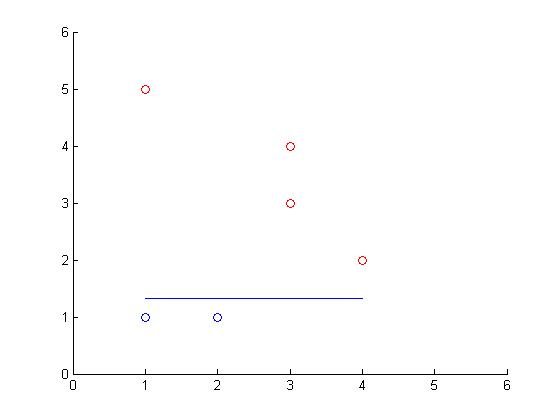
\includegraphics[width=0.65\textwidth]{hw3_1a}
\end{figure}

\item Part B:

Intuitively the hyperplane should be diagonal with a negative slope cutting through the positive and negative groups. Starting off, we can tell that point 4 will not be a support vector because if 3 is classified correctly, 4 will also be classified correctly. Point 6 will also not be a support vector because if 5 is classified correctly, 6 will be also. This leaves points 1, 2, 3, and 5 as support vectors with non-zero $\alpha$. Now, points 1, 3, and 2 form a line, $L_{123}$. Because they form a line, one of the points here is redundant. We will ignore point 1 and use 2 and 3 as support vectors. Since the hyperplane will be a straight line as well, the hyper plane must be parallel to $L_{123}$. A line is drawn parallel to $L_{123}$ intersecting point 5, $L_5$. The hyperplane should be placed half way between $L_{123}$ and $L_{5}$ parallel to both. $w_{opt}$ and $b_{opt}$ can be found geometrically as shown on the attached page at the end of this document.  

$w_{opt} = <1, 1>$ and $b_{opt} = -4.5$

The geometric margin can be found in the following manner:

$\gamma_{opt} = y_i*(w_{opt} \cdot x_i + b)/||w_{opt}||$

$||w_{opt}|| = (1^2+1^2)^{1/2} = 2^{1/2}$

For point 1,

$\gamma_{opt} = 1*(<1,1> \cdot <1,5> -4.5)/(2^{1/2}) = 1.0607 \approx 1$

This is consistent for all support vectors. Therefore, this is the optimal hyperplane.


\item Part C:

The modified biased perceptron algorithm nearly obtains the optimal weight vector and bias. The algorithm results were:

$w = <2,2>$ and $b = -8$

This corresponds to a hyperplane along the line $y = -x + 4$, which is very close to the optimal found in part b. The slopes are the same and the bias is off by $0.5$. 

Calculating the geometric margin for this hyper plane:

$\gamma_{opt} = y_i*(w_{opt} \cdot x_i + b)/||w_{opt}||$

$||w_{opt}|| = (2^2+2^2)^{1/2} = 8^{1/2}$

For point 1,

$\gamma_{opt} = 1*(<2,2> \cdot <1,5> -4)/(8^{1/2}) = 2.828$

For point 5,

$\gamma_{opt} = -1*(<2,2> \cdot <2,1> -4)/(8^{1/2}) = -0.707$

The geometric margin is not equal to the optimal geometric margin, so this is not the optimal hyperplane.


\begin{figure}[h!]
  \caption{Plot for Question 1, Part c}
  \centering
    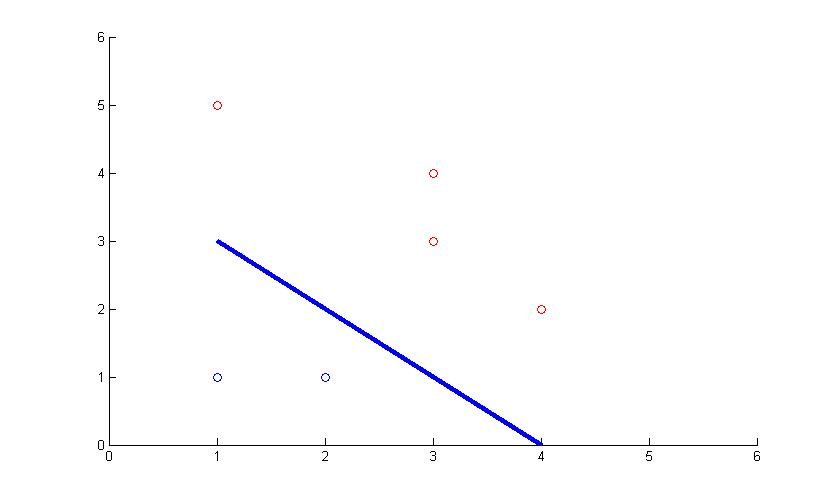
\includegraphics[width=0.65\textwidth]{hw3_1c}
\end{figure}

\newpage

\item Part D:

The $w_{opt}$ for $\gamma = 0.99$ is the closest to the optimal found in part b. In the graph below, the green line is the $w_{opt}$ for $\gamma = 0.99$ and the magenta line is the $w_{opt}$ found in part b.

\begin{figure}[h!]
  \caption{Plot for Question 1, Part d}
  \centering
    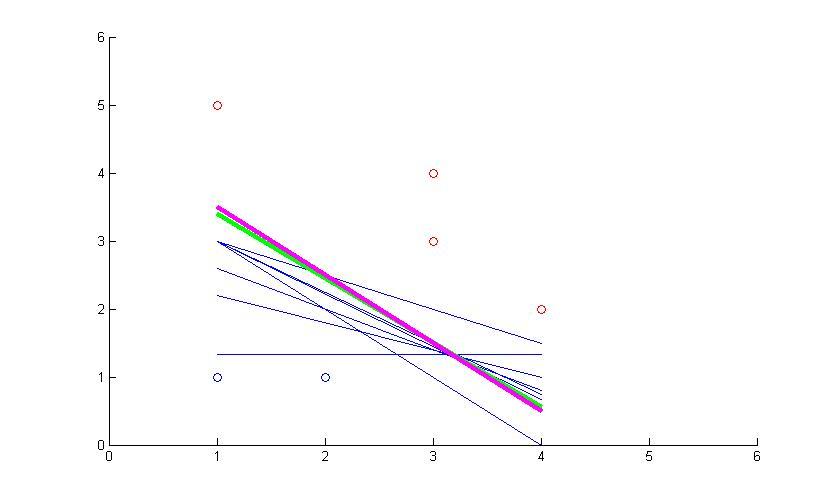
\includegraphics[width=1\textwidth]{hw3_1d2}
\end{figure}




\item Part E:

As beta increased the result became closer to the optimal weight vector and bias found in part b. Yes, this algorithm is a good alternative to an SVM for computing the optimal hyperplane because it is accurate and easy to implement. In part d, for $\gamma = 0.99$,

$w_{opt} = <36,38>$ and $b_{opt} = -165$

Calculating the geometric margin for the $w_{opt}$ for $\gamma = 0.99$,

$\gamma_{opt} = y_i*(w_{opt} \cdot x_i + b)/||w_{opt}||$

$||w_{opt}|| = (36^2+38^2)^{1/2} = 2740^{1/2}$

For point 1,

$\gamma_{opt} = 1*(<36,38> \cdot <1,5> -165)/(2740^{1/2}) = 1.165$

For point 5,

$\gamma_{opt} = -1*(<36,38> \cdot <2,1> -165)/(2740^{1/2}) = 1.051$

The geometric margins are very close to 1, which shows this solution is very close to optimal. This translates to a hyperplane on the line $y= -0.9474 + 4.3421$ which is very close to the optimal found in part b. The algorithm was also easy to implement and did not take long to run. The down side to this algorithm is that you need to know the geometric margin you want before you can run the algorithm.

\item Part F:

This algorithm converges after 100 iterations. The values for the weight vector and bias for more than 100 iterations is

$w = <7,9>$ and $b = -34$

For point 1,
$||w_{opt}|| = (7^2+9^2)^{1/2} = 130^{1/2}$

$\gamma_{opt} = 1*(<7,9> \cdot <1,5> -34)/(130^{1/2}) = 1.579$

This translates to a hyperlane along the line $y = -0.78x + 3.78$. For $\gamma = 0.9$, the optimal vectors from part c, primal, were:

$w = <7,9>$ and $b = -34$

This is the expected result because the primal and dual optimizations should produce the same result. The chart below shows the alpha values for each number of iterations.

\begin{figure}[h!]
  \caption{Plot for Question 1, Part f}
  \centering
    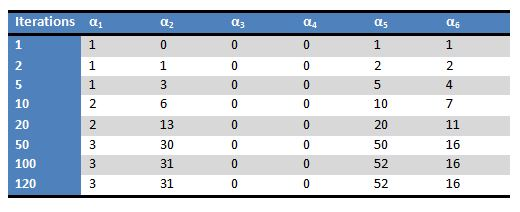
\includegraphics[width=1\textwidth]{hw3_1f}
\end{figure}

\newpage

\item Part G:

The following table shows the alpha values for three different gamma values. The alpha values have been normalized with the w vector such that $\alpha_i = \alpha_i'/||w||$ where $\alpha_i'$ is the raw alpha value.

\begin{figure}[h!]
  \caption{Plot for Question 1, Part g}
  \centering
    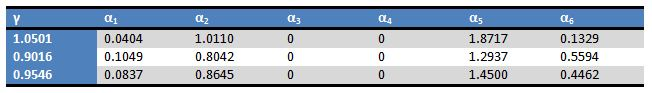
\includegraphics[width=1\textwidth]{hw3_1g}
\end{figure}

From this table we can determine the dominant support vectors for the positive and negative examples. Clearly 3 and 4 are not support vectors because there alpha values are zero, but by normalizing the alpha values we can see the relative importance of examples with non-zero alpha values. For example, $\alpha_1$ is very small compared to $\alpha_2$ and is never above 1. Example 2 is the dominant positive example. Similarly, $\alpha_5$ is much greater than $\alpha_6$. Therefore, the it seems the hyperplane would be mostly the same if only examples 2 and 5 were used. However, this is not the case when the program is run with only these two points. The result,

$w = <4,2>$ and $b = -15$

$\gamma_{opt} = 1*(<4,2> \cdot <1,5> -15)/(20^{1/2}) = -4.72$

Clearly this is not the correct hyperplane. If you were to connect points 2 and 5 with a straight line, find the midpoint, and draw a line perpendicular to the connecting line intersecting the midpoint, that line would not be the optimal hyperplane found in part b.

Using points 1, 2, and 5:

$w = <10,14>$ and $b = -15$

For point 1,

$\gamma_{opt} = 1*(<10,14> \cdot <1,5> -15)/(296^{1/2}) = 3.778$

This is still not the optimal hyperplane.

However, if point 3 were added, such that the only points were 2, 3, and 5, the result is,

$w = <6,6>$ and $b = -27$

For point 1,

$\gamma_{opt} = 1*(<6,6> \cdot <1,5> -27)/(72^{1/2}) = 1.061 \approx 1$

For point 3,

$\gamma_{opt} = 1*(<6,6> \cdot <3,3> -27)/(72^{1/2}) = 1.061 \approx 1$

Therfore, the support vectors are as dicussed in part b. The reason for the discrepancy could be the order in which the points are learned. Because point 3 is learned after points 1 and 2, it does not add any new information to the algorithm. 


\end{enumerate}

\section{Question 2}

\begin{enumerate}

\item Part A:

training error for class 1 = 0.0

training error for class 2 = 0.0

training error for class 3 = 0.0

training error for class 4 = 0.0

multiclass test error= 0.0970833333333


\item Part B:

for c = 0.125 multi\_class validation error= 0.063

for c = 0.125 multi\_class train error= 0.0

for c = 0.25 multi\_class validation error= 0.069

for c = 0.25 multi\_class train error= 0.0

for c = 0.5 multi\_class validation error= 0.068

for c = 0.5 multi\_class train error= 0.0

for c = 1.0 multi\_class validation error= 0.076

for c = 1.0 multi\_class train error= 0.0

for c = 2.0 multi\_class validation error= 0.077

for c = 2.0 multi\_class train error= 0.0

for c = 4.0 multi\_class validation error= 0.078

for c = 4.0 multi\_class train error= 0.0

for c = 8.0 multi\_class validation error= 0.078

for c = 8.0 multi\_class train error= 0.0

for c = 16.0 multi\_class validation error= 0.078

for c = 16.0 multi\_class train error= 0.0

for c = 32.0 multi\_class validation error= 0.078

for c = 32.0 multi\_class train error= 0.0

for c = 64.0 multi\_class validation error= 0.078

for c = 64.0 multi\_class train error= 0.0

for c = 128.0 multi\_class validation error= 0.078

for c = 128.0 multi\_class train error= 0.0

for c = 256.0 multi\_class validation error= 0.078

for c = 256.0 multi\_class train error= 0.0

for c = 512.0 multi\_class validation error= 0.078

for c = 512.0 multi\_class train error= 0.0

The graph below shows the multi-class validation error and multi-class training error as a function of log(C). The lowest validation error occurs when C = 0.125. Although the training error is not at its minimum, it is more important for the validation error be minimized. Therefore, the best C for the multi-class is 0.125. Normally, we would expect the best c parameter to be somewhere inside the range of c values observed. The best c parameter should occur at a valley of the validation error. There should be c parameters corresponding to higher validation error on either side of the best c parameter. This indicates that we should have looked at smaller values of c for this problem to verify that c = 0.125 is in fac the best parameter.

\begin{figure}[h!]
  \caption{Plot for Question 2, Part b}
  \centering
    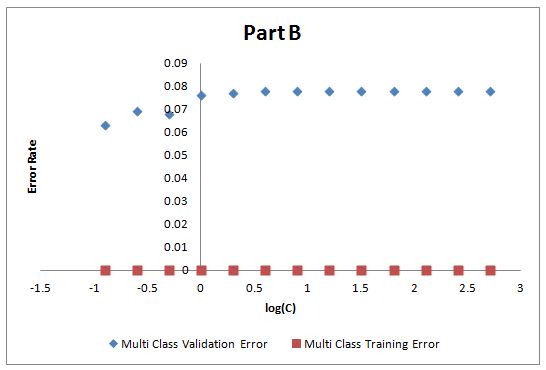
\includegraphics[width=0.75\textwidth]{hw3_2b}
\end{figure}

\newpage

\item Part C:

The best c value found in part b was c = 0.125. The results from part c for this c value are shown below.

test error for c=.125 soft margin= 0.08125

The multi-class test error for the soft margin algorithm is less than the multi-class test error for the hard margin in part a. In a hard margin classifier, a single outlier can determine the boundary. A soft margin classifier reduces the effect of noise on the data. A soft margin allows for more training error in order to improve the validation and test error.

\newpage

\item Part D:

Normalizing the data greatly impacts the results. For example, take a text classification with only two words of interest. The x-axis is the number of times the word "apple" is mentioned and the y axis the number of times the word "celery" is mentioned in the text. A text is classified as positive or negative. Suppose there are four example text as shown in the following plot. The red are positive and the blue are negative. The black line represent the general direction and location of the optimal hyperplane.

\begin{figure}[h!]
  \caption{Example: Not Normalized Data}
  \centering
    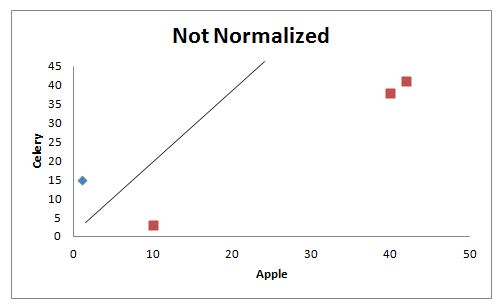
\includegraphics[width=0.4\textwidth]{notNormalized}
\end{figure}

\begin{figure}[h!]
  \caption{Example: Normalized Data}
  \centering
    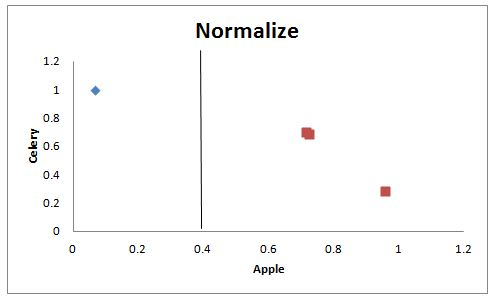
\includegraphics[width=0.4\textwidth]{normalized}
\end{figure}


When the data is normalized the data and hyperplane are shifted. This is because the two points that were in the top right corner are shifted. Although these points do not have a strong preference for apples or celery they have a large number of both. If, as in this example, the positive cases have very large numbers of both data, it could skew the set into classifying all points which have a very large number of either celery and apples into the positive class.

Results for Part D:



for c = 0.125 multi\_class validation error= 0.11

for c = 0.125 multi\_class train error= 0.0693333333333

for c = 0.25 multi\_class validation error= 0.07

for c = 0.25 multi\_class train error= 0.041

for c = 0.5 multi\_class validation error= 0.051

for c = 0.5 multi\_class train error= 0.0176666666667

for c = 1.0 multi\_class validation error= 0.045

for c = 1.0 multi\_class train error= 0.00733333333333

for c = 2.0 multi\_class validation error= 0.041

for c = 2.0 multi\_class train error= 0.001

for c = 4.0 multi\_class validation error= 0.043

for c = 4.0 multi\_class train error= 0.000333333333333

for c = 8.0 multi\_class validation error= 0.043

for c = 8.0 multi\_class train error= 0.0

for c = 16.0 multi\_class validation error= 0.045

for c = 16.0 multi\_class train error= 0.0

for c = 32.0 multi\_class validation error= 0.046

for c = 32.0 multi\_class train error= 0.0

for c = 64.0 multi\_class validation error= 0.046

for c = 64.0 multi\_class train error= 0.0

for c = 128.0 multi\_class validation error= 0.046

for c = 128.0 multi\_class train error= 0.0

for c = 256.0 multi\_class validation error= 0.046

for c = 256.0 multi\_class train error= 0.0

for c = 512.0 multi\_class validation error= 0.046

for c = 512.0 multi\_class train error= 0.0

The graph below shows the error after normalization. As was just explained the results are very different. Normalization is better becuase it reduces the effect that large data sets have on the results and reduces the effect of impurities. The best c value is 2.0 where the validation error is 0.041. This is a lower validation error than the minimum validation error from part b with the non-normalized data. 

\begin{figure}[h!]
  \caption{Plot for Question 2, Part d}
  \centering
    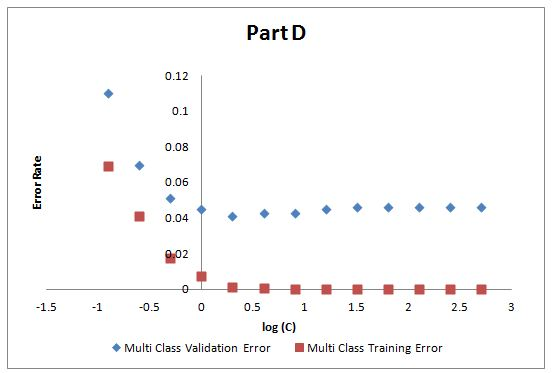
\includegraphics[width=1\textwidth]{hw3_2d}
\end{figure}

Furthermore, normalization also improves the results from part c in which the entire training data set was used to train. The soft margin multiclass error when using the entire normalized training set was found to be 0.0675. This is smaller than the soft margin multi-class error found in part c, 0.08125.

\newpage

\item Part E:



for c = 0.125 multi\_class validation error= 0.155

for c = 0.125 multi\_class train error= 0.137666666667

for c = 0.25 multi\_class validation error= 0.1

for c = 0.25 multi\_class train error= 0.0786666666667

for c = 0.5 multi\_class validation error= 0.068

for c = 0.5 multi\_class train error= 0.034

for c = 1.0 multi\_class validation error= 0.046

for c = 1.0 multi\_class train error= 0.0133333333333

for c = 2.0 multi\_class validation error= 0.036

for c = 2.0 multi\_class train error= 0.00266666666667

for c = 4.0 multi\_class validation error= 0.036

for c = 4.0 multi\_class train error= 0.000333333333333


for c = 8.0 multi\_class validation error= 0.041

for c = 8.0 multi\_class train error= 0.0

for c = 16.0 multi\_class validation error= 0.042

for c = 16.0 multi\_class train error= 0.0

for c = 32.0 multi\_class validation error= 0.042

for c = 32.0 multi\_class train error= 0.0

for c = 64.0 multi\_class validation error= 0.042

for c = 64.0 multi\_class train error= 0.0

for c = 128.0 multi\_class validation error= 0.042

for c = 128.0 multi\_class train error= 0.0

for c = 256.0 multi\_class validation error= 0.042

for c = 256.0 multi\_class train error= 0.0

\begin{figure}[h!]
  \caption{Example: Normalized Data}
  \centering
    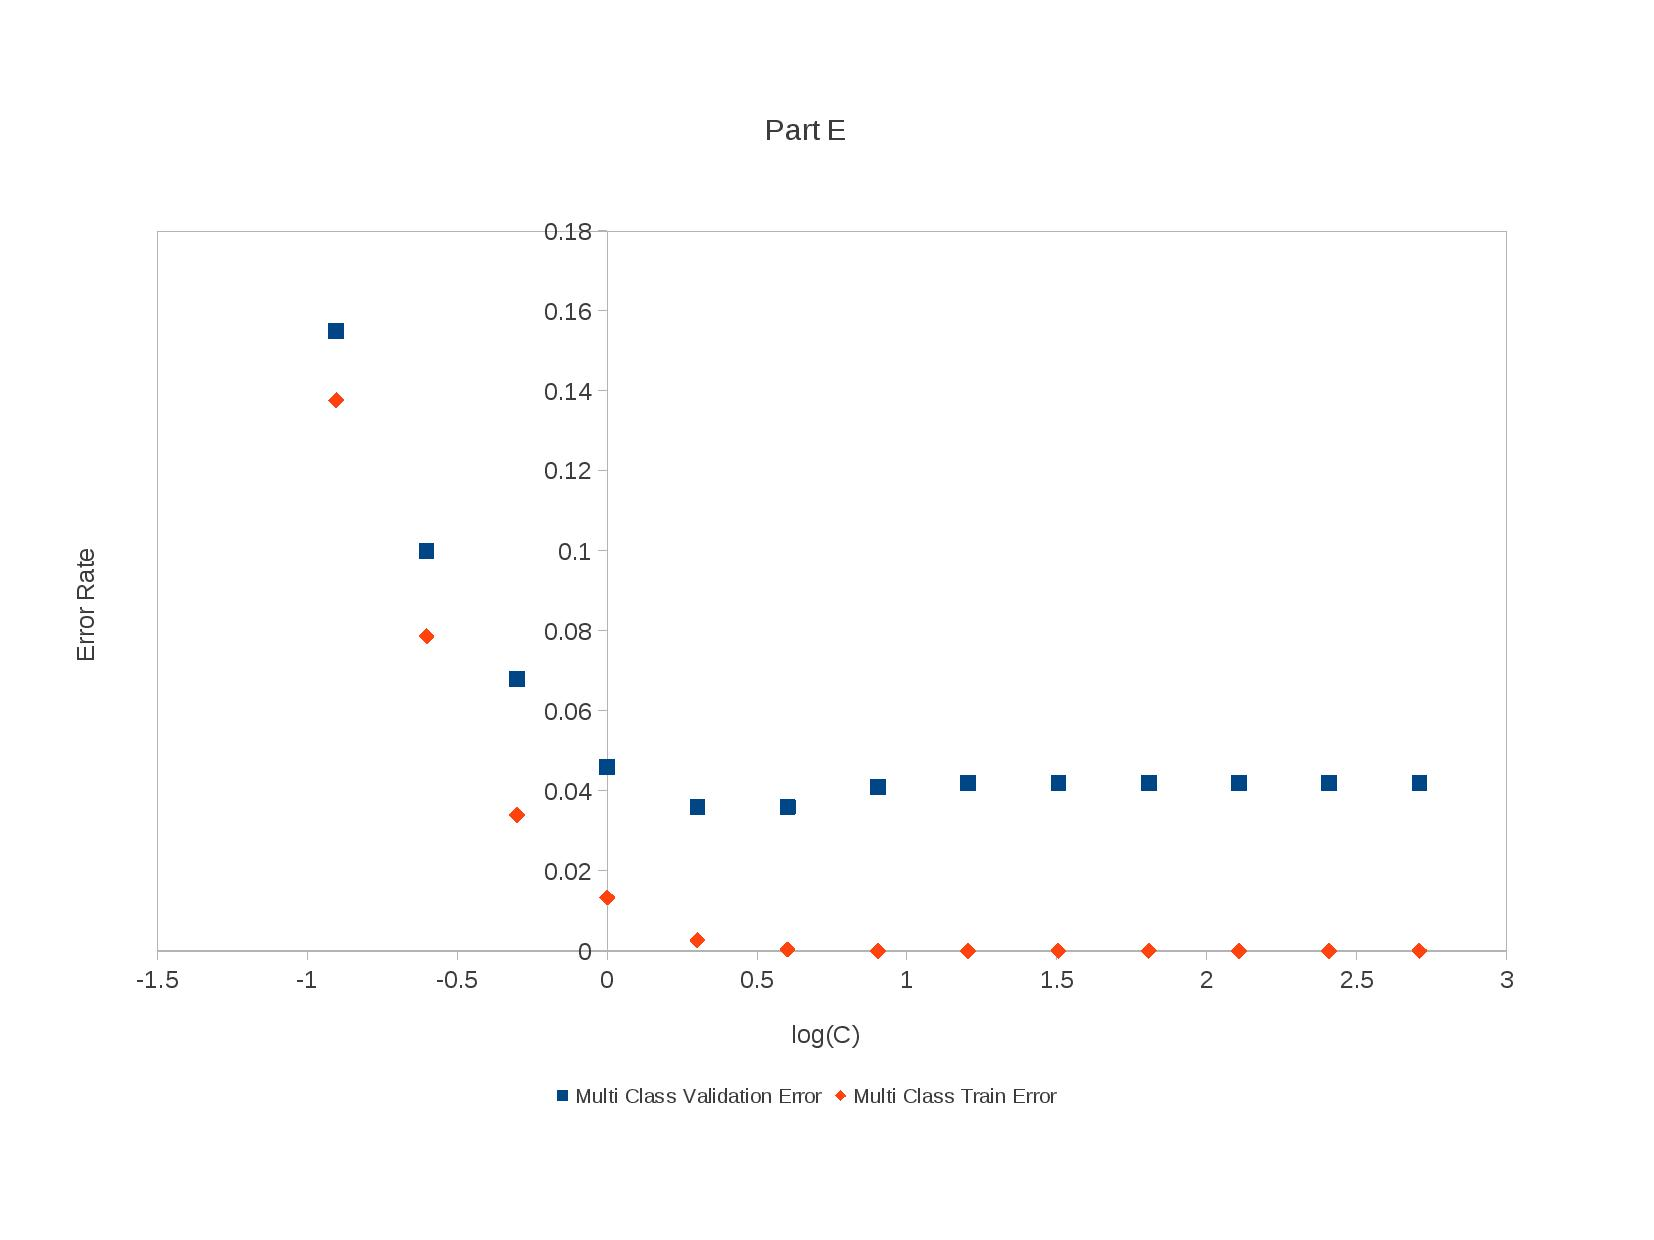
\includegraphics[width=1\textwidth]{hw3_2e}
\end{figure}

The best c parameter is c = 2.0 or c = 4.0 when the validation error is 0.036. This validation is slightly better than that found for part d (1 v all).

The soft margin multi class test errors for c = 2.0 are:

1 vs 1:	0.136666666667

1 vs all: 	0.0675

Thus, the accuracies are:

1 vs 1: $1-0.136666666667 = 0.863$

1 vs all: $1-0.675 = 0.9325$

The 1 vs all method is more accurate than the 1 vs 1 method.


The running times are as follows:

Running Time (1 vs 1) = 39.245677948 seconds

Running Time (1 vs all) = 84.2226040363 seconds

Using the python stopwatch script, we found that the 1 vs all method takes over twice as much time to run as the 1 vs 1 method as shown above. The most expensive task is learning followed by classifying and then voting. The 1 vs 1 method has 6 classes each with approximately $750*2$ examples, 750 positive and 750 negative. 1 vs all has 4 classes each with approximately $750*4$ examples. The total number of examples for the 1 vs 1 is approximately $12*750$ whereas the total number of examples for 1 vs all is approximately $16*750$. The total size of the classes for 1 vs all is $4/3$ as large as the 1 vs 1 method. This means that the 1 vs all case will need to learn $1/3$ more examples than the 1 vs 1 method. Therefore the running time for 1 vs 1 should be about $4/3$ as long as the running time for 1 vs all based on the number of examples to learn.


\end{enumerate}
\section{READ ME}


For Question 1, open the code in MatLab for each part and click run. The name of the code indicates which part it is for. No additional inputs or libraries are needed.

For Question 2, save all python files into one folder. In the folder containing the folder containing the python files, save the test and train documents. To run the code, type "python *.py" into the terminal (for Linux users). Replace the star witht the name of the program for the given part listed below.


\section{Code}

\begin{lstlisting}
% Homework 3 Problem 1 Part A
clc
clear all
points = [1 4 3 3 2 1;
          5 2 3 4 1 1;
          1 1 1 1 1 1];
y = [1 1 1 1 -1 -1];
   


w =[0; 0; 0];
k = 0;
done = false;


while ~done
    thisLoop = 0;
    for i = 1:6
        if y(i)*dot(w,points(:,i)) <= 0
           w = w + y(i)*points(:,i);
           k=k+1;
           thisLoop = thisLoop +1;
        end
    end
    
    if thisLoop == 0
        done = true;
    end
    
end

x_pos = [1 3 3 4];
y_pos = [5 4 3 2];
x_neg = [1 2];
y_neg = [1 1];
hold on
scatter(x_pos,y_pos,'r')
scatter(x_neg,y_neg,'b')
refline(-w(1)/w(2),-w(3)/w(2))

axis([0 6 0 6])
hold off

%%%%%%%%%%%%%%%%%%%%%%%%%%%%%%%%%%%%%%%
Question 1 Part C

clc
clear all
points = [1 4 3 3 2 1;
          5 2 3 4 1 1;
          1 1 1 1 1 1];
y = [1 1 1 1 -1 -1];

gamma_opt = (3/4)*sqrt(2);


gamma = 0.5*gamma_opt;
done = false;
k = 0;
w = [0;0;0];
while ~done
    thisLoop = 0;
    for i = 1:6
        if k == 0
           w = w + y(i)*points(:,i);
           k=k+1;
           thisLoop = thisLoop +1;
        elseif (y(i)*dot(w,points(:,i)))/norm(w(1:2)) < gamma
           w = w + y(i)*points(:,i);
           k=k+1;
           thisLoop = thisLoop +1;
        end
    end
    
    if thisLoop == 0
        done = true;
    end
    
end
w
x_pos = [1 3 3 4];
y_pos = [5 4 3 2];
x_neg = [1 2];
y_neg = [1 1];
hold on
scatter(x_pos,y_pos,'r')
scatter(x_neg,y_neg,'b')
refline(-w(1)/w(2),-w(3)/w(2))
axis([0 6 0 6])

hold off

%%%%%%%%%%%%%%%%%%%%%%%%%%%%%%%%%%
%% Question 1 Part D

clc
clear all
points = [1 4 3 3 2 1;
          5 2 3 4 1 1;
          1 1 1 1 1 1];
y = [1 1 1 1 -1 -1];

gamma_opt = (3/8)*sqrt(2);

beta = [0.1 0.2 0.3 0.4 0.5 0.6 0.7 0.8 0.9 0.94 0.99];
w_final = zeros(3,length(beta));

for j = 1:length(beta)
    gamma = beta(j)*gamma_opt;

    w =[0; 0; 0];
    k = 0;
    done = false;
    iterations = 0;
    while ~done
        thisLoop = 0;
        for i = 1:6
            if k == 0
               w = w + y(i)*points(:,i);
               k=k+1;
               thisLoop = thisLoop +1;
            elseif (y(i)*dot(w,points(:,i)))/norm(w(1:2)) < gamma
               w = w + y(i)*points(:,i);
               k=k+1;
               thisLoop = thisLoop +1;
            end
        end
        %iterations = iterations +1;
        if thisLoop == 0 %|| iterations == 10000
            done = true;
        end

    end
    w_final(:,j) = w;
end

w_final
x_pos = [1 3 3 4];
y_pos = [5 4 3 2];
x_neg = [1 2];
y_neg = [1 1];
hold on
scatter(x_pos,y_pos,'r')
scatter(x_neg,y_neg,'b')
% refline(0,4/3)
% refline(-1/2,7/2)
% refline(-1,4)
for n = 1:length(beta)
    m = -w_final(1,n)/w_final(2,n);
    b = -w_final(3,n)/w_final(2,n);
    refline(m,b)
end

axis([0 6 0 6])

hold off

%%%%%%%%%%%%%%%%%%%%%%%%%%%%%%%%%%
Question 1 Part F

clc
clear all
points = [1 4 3 3 2 1;
          5 2 3 4 1 1;
          1 1 1 1 1 1];
y = [1 1 1 1 -1 -1];


gamma_opt = (3/4)*sqrt(2);

beta = .9;

a = zeros(1,6);

gamma = beta*gamma_opt

done = false;
iterations = 0;
flag = 1;
while ~done
    
    for i = 1:6       
        
        w = [0; 0; 0];
        for k = 1:length(a)                
            w = w + a(k)*y(k)*points(:,k); 
        end
        
        if y(i)*dot(w,points(:,i))/norm(w(1:2)) <= gamma || flag == 1
            flag = 0;
            a(i) = a(i) + 1;
        end
    end
    iterations = iterations + 1;
    if iterations == 1000
        
        done = true;
    end

end

%%%%%%%%%%%%%%%%%%%%%%%%%%%%%%%%%%%%%%%%%%%%%%
Question 2:

General Code used throughout;


%%%%%%%%%%%%%%%%%%%%%%%%%%%%%%%%%%%%%%%%%%%%%%
def parse(file_name):
    file = open(file_name)
    train= []
    for line in file:
        has_class= False
        current_example= None
        for s in line.split():
            if not has_class:
                my_class= int(s)
                current_example= (my_class, [])
                train.append(current_example)
                has_class= True
            else:
                word, frequency= [int(t) for t in s.split(":")]
                current_example[1].append((word, frequency))

    file.close
    return train
%%%%%%%%%%%%%%%%%%%%%%%%%%%%%%%%%%%%%%%%%%%%%%
Part A:

parta.py:

from parser import parse
from parta_funcs import find_single_class_error, find_multiclass_error, find_models

tst= parse("../articles.test")
trn= parse("../articles.train")
mdls= find_models(trn, 1024)

for i in range(len(mdls)):
    print "training error for class " + str(i+1) +" = " + \
            str(find_single_class_error(mdls[i], trn, i+1))

print "multiclass test error= " + str(find_multiclass_error(mdls, tst))

parta_funcs.py:

from parser import parse
import svmlight


def predict_classification(classifications, example):
    best_value= classifications[0][example]
    best_index= 0
    for classification_index in range(len(classifications)):
        if classifications[classification_index][example] > best_value:
            best_value= classifications[classification_index][example]
            best_index= classification_index

    return best_index+1

def find_multiclass_error(models, test):
    errors= 0
    classifications= []
    for i in range(len(models)):
        classifications.append(svmlight.classify(models[i], test))

    for i in range(len(test)):
        predicted_classification= predict_classification(classifications, i)
        if predicted_classification != test[i][0]:
 	errors= errors+1

    return float(errors)/len(test)

def find_single_class_error(model, test, target_example):
    errors= 0
    test= change_to_binary_examples(test, target_example)
    classification= svmlight.classify(model, test)
    for i in range(len(test)):
        predicted_classification= 0
        if(classification[i] > 0):
            predicted_classification= 1
        else:
            predicted_classification= -1

	if predicted_classification != test[i][0]:
           errors= errors+1

    return float(errors)/len(test)

def change_to_binary_examples(training_data, target_example):
    binary= []
    for i in range(len(training_data)):
        if training_data[i][0] == target_example:
            binary.append((1, training_data[i][1]))
        else:
            binary.append((-1, training_data[i][1]))

    return binary


def find_models(training_data, c_value):
    models= []
    for i in range(1,5):
        train= change_to_binary_examples(training_data, i)
	models.append(svmlight.learn(train, type='classification', C=c_value))

    return models

%%%%%%%%%%%%%%%%%%%%%%%%%%%%%%%%%%%%%%%%%%%%%%%%
Part B:

partb.py:

from parser import parse
from partb_funcs import find_multiclass_validate_and_train_error

train= parse("../articles.train")
find_multiclass_validate_and_train_error(train)

partb_funcs.py

import random
from parser import parse
from parta_funcs import find_multiclass_error, find_models

def create_validate_and_train_subsets(train):
    random.shuffle(train)

    train_subset= []
    validate_subset= []

    i= 0

    while i < len(train)*.75:
        train_subset.append(train[i])
        i= i+1

    while i < len(train):
        validate_subset.append(train[i])
        i= i+1

    return train_subset, validate_subset

def find_multiclass_validate_and_train_error(train):
    train_subset, validate_subset= create_validate_and_train_subsets(train)
    for c in [.125 * 2**j for j in range(13)]:
        models= find_models(train_subset, c)
        print "for c = " + str(c) + " multi_class validation error= " + \
        str(find_multiclass_error(models, validate_subset))

        print "for c = " + str(c) + " multi_class train error= " + \
        str(find_multiclass_error(models, train_subset))

%%%%%%%%%%%%%%%%%%%%%%%%%%%%%%%%%%%%%%%%%%%%%%%%%%
Part C:

partc.py:

import random
from parser import parse
from parta_funcs import find_multiclass_error, find_models

train= parse("../articles.train")
test= parse("../articles.test")

i= 0

models= find_models(train, .125)

print "test error for c=.125 soft margin= " + \
        str(find_multiclass_error(models, test))

%%%%%%%%%%%%%%%%%%%%%%%%%%%%%%%%%%%%%%%%%%%%%%%%%%
Part D:

partd.py:

from parser import parse
from partd_funcs import normalize
from partb_funcs import find_multiclass_validate_and_train_error
import stopwatch

t = stopwatch.Timer()

train= parse("../articles.train")
train= normalize(train)
find_multiclass_validate_and_train_error(train)

print "Running Time = " + str(t.elapsed)


partd_funcs.py:

import math

def normalize(examples):
    normalized_examples= []
    for ex in examples:
        features= ex[1]
        div= math.sqrt(reduce(lambda x, y: x+y[1]**2, features, 0))
        normalized_features= []
        for feat in features:
            normalized_features.append((feat[0], feat[1]/div))
        normalized_examples.append((ex[0],normalized_features))

    print str(math.sqrt(reduce(lambda x, y: x+y[1]**2,
                                    normalized_examples[0][1], 0)))
    return normalized_examples

partc_norm.py:

import random
from parser import parse
from parta_funcs import find_multiclass_error, find_models
from partd_funcs import normalize

train= parse("../articles.train")
train = normalize(train)
test= parse("../articles.test")

i= 0

models= find_models(train, 2)

print "test error for c=2 soft margin= " + \
        str(find_multiclass_error(models, test))

%%%%%%%%%%%%%%%%%%%%%%%%%%%%%%%%%%%%%%%%%%%%%%%%

Part E:

parte.py: 

from parser import parse
from parte_funcs import onevone_multiclass_validate_and_train_error
import stopwatch

t = stopwatch.Timer()

train= parse("../articles.train")
onevone_multiclass_validate_and_train_error(train)

print "Running Time = " + str(t.elapsed)


parte_funcs.py:

import svmlight
import random
from partd_funcs import normalize
from partb_funcs import create_validate_and_train_subsets

def make_1v1_examples(training_data, positive_example, negative_example):
    onevone= []
    for example in training_data:
        if example[0] == positive_example:
            onevone.append((1, example[1]))
        elif example[0] == negative_example:
            onevone.append((-1, example[1]))

    return onevone

def find_1v1_models(training_data, c_value):
    models= {}
    for i in range(1,5):
        for j in range(i+1,5):
            train= make_1v1_examples(training_data, i, j)
            models[(i,j)]= \
            svmlight.learn(train, type='classification', C=c_value)
    return models

def predict_classification_1v1(classifications, i):
    votes= {}
    for pair in classifications.keys():
        if classifications[pair][i] > 0:
            if pair[0] in votes:
                votes[pair[0]]= votes[pair[0]] + 1
            else:
                votes[pair[0]]= 1
        else:
            if pair[1] in votes:
                votes[pair[1]]= votes[pair[1]] + 1
            else:
                votes[pair[1]]= 1

    max_vote_num = max(votes.values())

    highest_votes= {}

    for class_num in votes.keys():
        if votes[class_num] == max_vote_num:
            highest_votes[class_num] = 1

    for vote_weight in highest_votes.values():
        vote_weight= float(vote_weight)/len(highest_votes)

    return highest_votes

def multiclass_error_1v1(models, test):
    errors= 0
    classifications= {}
    for pair in models.keys():
        classifications[pair]=(svmlight.classify(models[pair], test))

    for i in range(len(test)):
        votes= predict_classification_1v1(classifications, i)
        for classNum in range(1,5):
            if classNum in votes and test[i][0] != classNum:
                errors= errors + votes[classNum]

    return float(errors)/len(test)

def onevone_multiclass_validate_and_train_error(train):
    train= normalize(train)
    train_subset, validate_subset= create_validate_and_train_subsets(train)
    for c in [.125 * 2**j for j in range(13)]:
        models= find_1v1_models(train_subset, c)
        print "for c = " + str(c) + " multi_class validation error= " + \
                str(multiclass_error_1v1(models, validate_subset))
        print "for c = " + str(c) + " multi_class train error= " + \
                str(multiclass_error_1v1(models, train_subset))


parte2.py:

from parte_funcs import multiclass_error_1v1, find_1v1_models
from parser import parse

train= parse("../articles.train")
test= parse("../articles.test")

models= find_1v1_models(train, 2)

print "test error for c=2 soft margin= " + \
        str(multiclass_error_1v1(models, test))


stopwatch.py:
*This was downloaded from http://code.google.com/p/7oars/downloads/detail?name=stopwatch-0.3.1-py2.5.egg&can=2&q=


\end{lstlisting}

\end{document}